\documentclass[review]{elsarticle}
\usepackage{amssymb}
%\usepackage{graphicx}
\usepackage{amsmath}
\usepackage{color}
%\usepackage{tikz}
%\usetikzlibrary{arrows,shapes}
%\usetikzlibrary{shapes.geometric}
%\usetikzlibrary{arrows.meta}
\usepackage{authblk}
\usepackage{graphics,graphicx}
\usepackage{mathrsfs}
\usepackage{amsmath,bm}
\usepackage{subfigure}
\usepackage{booktabs}
\usepackage{amsthm}
\usepackage{subfigure}
\usepackage{listings}
\usepackage{setspace}
\graphicspath{{picture/}}
\graphicspath{{TikzFig/}}

%\journal{Journal of Computational Physics}
\bibliographystyle{elsarticle-num}

\begin{document}

\title{A multi-material HLLC Riemann solver with both elastic and plastic waves for 1D  elastic-plastic flows}
\author{Li Liu$^1$, Jun-bo Cheng $^{1,*}$, Jiequan Li $^{1}$}
%\cortext[mycorrespondingauthor]{
%Correspondence to: Junbo Cheng, Institute of Applied Physics and Computational Mathematics, Beijing 100094, China. E-mail: Cheng\_junbo@iapcm.ac.cn}

\maketitle

\address{$^1$  Institute of Applied Physics and Computational Mathematics, Beijing 100094, China }

\begin{abstract}
  A multi-material HLLC-type  approximate Riemann solver with both elastic and plastic waves (MHLLCEP) is constructed for 1D elastic-plastic flows with the  hypo-elastic model and the von Mises yielding condition. Although Cheng in 2016 introduced a HLLC Riemann solver with elastic waves(HLLCE) for 1D elastic-plastic flows, Cheng assumed that pressure is continuous across the contact wave. This assumption maybe lead to big errors, especially for multi-material elastic-plastic flows. In our MHLLCEP, this assumption is not used again, and correspondingly the errors introduced by the assumption are deleted, describing and evaluating the plastic waves are more accurate than that in the HLLCE. Moreover, if the non-linear waves in the Riemann problem are only shock waves, even with the plastic waves, our MHLLCEP is theoretically accurate. For  the multi-material system, in this paper, a ghost cell method is used to achieve a high-order spatial reconstruction across the interface without numerical oscillations. Based on the MHLLCEP, combining with the third-order WENO reconstruction method and the third-order Runge-Kutta method in time, a high-order cell-centered Lagrangian scheme for 1D multi-material elastic-plastic flows is built in this paper. A number of numerical experiments are carried out. Numerical results show  that the presented third-order scheme is convergent, robust, and essentially non-oscillatory. Moreover, for multi-material elastic-plastic flows, the scheme with  the MHLLCEP is more accurate and reasonable in resolving the multi-material interface than the scheme with the  HLLCE.
\end{abstract}

\begin{keyword}
  HLLC Riemann solver, high-order cell-centered Lagrangian scheme,  WENO scheme,  hypo-elastic model, elastic-plastic flows
\end{keyword}

%\end{frontmatter}

\section{Introduction}

In this paper, a multi-material elastic-plastic HLLC-type approximate Riemann solver(MHLLCEP) is developed, with the capability of resolving both elastic and plastic waves, to simulate one-dimensional  multi-material elastic-plastic solid problems with the isotropic elastic-plastic model \cite{wilkins1963calculation} and  the von Mises' yielding condition in the framework of the  high-order cell-centered Lagrangian scheme.

Generally, elastic-plastic flows can be mainly simulated in three ways, Eulerian methods \cite{trangenstein1991higher,miller2001high,barton2009exact}, staggered Lagrangian schemes \cite{wilkins1963calculation} and cell-centered Lagrangian schemes \cite{burton2013cell,kluth2010discretization,maire2013nominally,cheng2017third} that  is considered in this paper. Comparing with the staggered Lagrangian scheme, cell-centered Lagrangian  schemes  have many advantages. Firstly, it's no necessary to add  extra artificial viscosity  which  must be used in the staggered Lagrangian schemes; Secondly, it is easy to guarantee the total energy conservation; Besides, it can also be used to simulate the problems with both  hyper-elastic and hypo-elastic models  \cite{burton2013cell,kluth2010discretization,maire2013nominally,cheng2017third}  as a Lagrangian scheme.

%In the  Godunov-type method
For a cell-centered Lagrangian scheme, a core process is to move the node of grids with the speed of fluids
 % and to construct the conservative flux
 by solving a Riemann problem at each cell face. As the Riemann problem contains many physical structures, especially in elastic-plastic flows, such as elastic waves, plastic waves and contact waves
  %or interfaces between different materials
  , the property of the approximate Riemann solver is of great importance in the simulation. Recently, a lot of works have been done in
  this area. For example, Gavrilyuk et al. \cite{gavrilyuk2008modelling} analyzed the structure of the Riemann solution and construct a Riemann solver for the linear elastic system  of hyperbolic non-conservative models for transverse waves, wherein, an extra evolution equation was added in order to make the elastic transformations reversible in the absence of shock waves. Despres \cite{despres2007geometrical} built a shock solution to a non-conservations reversible system of hypo-elasticity models and found that a sonic point is necessary to construct  the compression solution that begins at a constrained compressed state.  Cheng et al.  \cite{cheng2015high} analyzed the wave structures of one-dimensional elastic-plastic flows and developed an effective two-rarefaction approximate Riemann solver with elastic waves (TRRSE) and built a  second-order and  a third-order cell-centered Lagrangian schemes based on the TRRSE, but the TRRSE is a little  expensive as  the iteration method is used.
In \cite{cheng2016harten}, for one-dimensional elastic-plastic flows, Cheng introduced a HLLCE Riemann solver, which is fast and efficient in resolving elastic waves and plastic waves. In the HLLCE,  Cheng evaluated the deviatoric stresses from the following \emph{assumption: a pressure is continuous across the contact wave}. This assumption is valid for pure fluids, but  in  elastic-plastic flows, this assumption may lead to some errors. There are three cases we need  to consider.
\begin{enumerate}
  \item If states in the star regions on both sides of the contact wave are elastic, this assumption does not result in errors;
  \item If both states reach the elastic limit, there are two cases need  to be taken into account:
  \begin{enumerate}
    \item if both  materials in both sides of the interface are same, this assumption does not result in errors either.
    \item if  materials are different, this assumption will result in big errors because the yielding strengths of different materials are different;
  \end{enumerate}
  \item If one state in one side of the interface reaches the elastic limit, but another is  not,  this assumption will  also result in big errors.
\end{enumerate}

%For above considerations,
In this paper, in order to eliminate these errors,
 we want to construct a new HLLC-type Riemann solver for 1D multi-material elastic-plastic flows. In the new solver, both the elastic waves and plastic waves are correctly resolved and the assumption in \cite{cheng2016harten} that the pressure is continuous across the interface is deleted; Correspondingly, the errors introduced by the assumption will also be eliminated.

Based on the MHLLCEP, we develop a high-order elastic-plastic cell-centered Lagrangian scheme for one-dimensional multi-material elastic-plastic flows. If we directly use the WENO reconstruction method \cite{liu2018novel} for multi-material elastic-plastic problems,
%With a high-order reconstruction scheme,
the spacial stencil may cross the material interface
% and in a multi-material state, and  will cause oscillation
 and numerical oscillations may be caused near the interface. In order to delete the numerical oscillations neat the material interface, a ghost cell method is used
   %in the  multi-material system to obtain a stable high-order reconstruction.
   Combined with an improved third-order WENO scheme\cite{liu2018novel} and the third-order Runge-Kutta scheme, a high-order cell-centered Lagrangian scheme is given in this paper for one-dimensional multi-material elastic-plastic flows.

This paper is organized as follows. In section 2, we briefly introduce the governing equations to be studied. In section 3, the MHLLCEP method is constructed.  Then, high-order elastic-plastic cell-centered Lagrangian scheme is given in section 4. Some numerical examples are presented to validate the method.  Conclusions are shown in section 5.

\section{Governing equations}
In this paper, the elastic energy is not included in the total energy. The exclution of the elastic energy is usual for practical engineering problems \cite{maire2013nominally} and is different from that in Ref.\cite{gavrilyuk2008modelling}.

The governing equations system is given as 
 \begin{equation}\label{eq:1d}
   \left\{ \begin{aligned}
       & \partial _t \rho +\partial_x(\rho u)=0,\\
       & \partial _t (\rho u)+\partial_x(\rho u^2 + p -s_{xx})=0,\\
       &\partial _t (\rho E)+\partial_x\left[(\rho E + p -s_{xx})u\right]=0,\\
       &\partial _t s_{xx}+u\partial_xs_{xx}-\frac{4}{3}\partial_x u=0,\\
& |s_{xx}|\leq \frac{2}{3}Y_{0}, \\
        \end{aligned}
  \right.
\end{equation}
It contains the following parts. 

\subsection{Conservation terms}
For  the  continuous one-dimensional solid, the conservation terms  in differential form can be  given as
\begin{equation*}
\partial_t \mathbf{{U}} + \partial _x \bm{F}(\mathbf{{U}}) = 0, \   x \in \   \Omega \subset \mathbf{R}, \  t>0,
\end{equation*}
where
\begin{equation}
  \mathbf{U} = \left[ \begin{array}{l}
      \rho \\
      \rho u \\
      \rho  E \\
    \end{array}
  \right],
  \hspace{0.3cm}
  \mathbf{F} = \left[ \begin{array}{l}
      \rho u \\
      \rho u^2 -\sigma\\
      (\rho E -\sigma)u\\
  \end{array} \right],
\end{equation}
$\rho$, $u$, $\sigma$ and $E$ are  the density, velocity in $x-$direction, Cauchy stress and total energy per unit volume, respectively, $E$ has the relation with specific internal energy $e$ as
\begin{equation}
  E = e+\frac{1}{2}u^2,
\end{equation}
\begin{equation}
  \sigma = -p +s_{xx},
\end{equation}
where $p$ and $s_{xx}$ denote hydrostatic pressure and deviatoric stress in the $x-$ direction, respectively.

\subsection{The equation of state (EOS)}

The relation of the pressure with  the density and the specific internal energy is gotten from the equation of state (EOS). In this paper, we consider the Mie-Gr\"uneisen EOS,
\begin{equation}\label{eq:mie}
  p(\rho,e) = \rho_0 a_0^2f(\eta)+ \rho_0 \Gamma_0 e,
\end{equation}
where $f(\eta) = \frac{(\eta-1)(\eta-\Gamma_0(\eta-1)/2)}{(\eta-s(\eta-1))^2}$, $\eta = \frac{\rho}{\rho_0}$, $\rho_0$, $a_0$, $s$ and $\Gamma_0$ are constant parameters of the Mie-Gr\"uneisen EOS.

\subsection{The constitutive relation}
Hooke's law is used here to describe the relationship between the deviatoric stress and the strain,
\begin{equation}\label{eq:sxx1}
\dot{s}_{xx} = 2\mu \left(\dot{\varepsilon}_x-\frac{1}{3}\frac{\dot{V}}{V}\right),
\end{equation}
where $\mu$ is the shear modulus, $V$ is the volume, and the dot means the material time derivative,
\begin{equation}\label{eq:mt}
  \dot{()} = \frac{\partial ()}{\partial t} + u \frac{\partial ()}{\partial t},
\end{equation}
and
\begin{equation}\label{eq:vare}
  \dot{\varepsilon}_x = \frac{\partial u}{\partial x}, \hspace{0.3cm} \frac{\dot{V}}{V} = \frac{\partial u}{\partial x}.
\end{equation}

By using Eq.(\ref{eq:vare}), Eq.(\ref{eq:sxx1}) can be rewritten as
\begin{equation}\label{eq:sxx}
  \frac{\partial s_{xx}}{\partial t} + u \frac{\partial s_{xx}}{\partial t} =\frac{4}{3}\mu \frac{\partial u}{\partial x}.
\end{equation}

\subsection{The yielding condition}
The Von Mises' yielding condition is used here to describe the elastic limit. In one spatial dimension, the von Mises' yielding criterion is given by
\begin{equation}
  |s_{xx}| \le \frac{2}{3}Y_0,
\end{equation}
where $Y_0$ is the yield strength of the material in simple tension.

\section{The Riemann problem}


The Riemann problem for the 1D time dependent elastic-plastic equations is given as follows:
 \begin{equation}\label{eq:1d}
   \left\{ \begin{aligned}
       & \partial _t \rho +\partial_x(\rho u)=0,\\
       & \partial _t (\rho u)+\partial_x(\rho u^2 + p -s_{xx})=0,\\
       &\partial _t (\rho E)+\partial_x\left[(\rho E + p -s_{xx})u\right]=0,\\
       &\partial _t s_{xx}+u\partial_xs_{xx}-\frac{4}{3}\partial_x u=0,\\
& |s_{xx}|\leq \frac{2}{3}Y_{0}, \\
       &Q(x,t = 0) = \left\{\begin{aligned}
           Q_L, \hspace{0.1cm} \text{if} \hspace{0.1cm} x<0, \\
           Q_R, \hspace{0.1cm} \text{if} \hspace{0.1cm} x\ge 0, \\
       \end{aligned}\right.
     \end{aligned}
  \right.
\end{equation}
where $Q = (\rho, \rho u, \rho E, s_{xx})^T$.

According to the yielding of the material, the euqations may have different Jacobian matrix and different sonic velocities. We will discuss them seprately.
\subsection{Jacobian matrix in  elastic regions} %and the eigenvalues and eigenvectors}
For the Mie-Gr\"uneisen EOS, if the material is not yielding and 
\begin{equation}
  |s_{xx}| < \frac{2}{3}Y_0,
\end{equation}
the system (\ref{eq:1d}) can be written as
\begin{equation}
 \partial_t \mathbf{Q} +\mathbf{J}(\mathbf{{Q}})\partial_x\mathbf{Q} = 0,
\end{equation}
where $Q = (\rho, \rho u, \rho E, s_{xx})$, and the Jacobian matrix is 
\begin{equation}\label{eq:Jcb}
  J(Q) = \left[\begin{array}{llll}
      0 & 1 & 0 & 0 \\
      -u^2 + \frac{\partial p}{\partial \rho} +\Gamma(\frac{u^2}{2}-e)& u(2-\Gamma)& \Gamma & -1 \\
	  (\Gamma(\frac{u^2}{2}-e)-e-\frac{u^2}{2}+\frac{\sigma}{\rho}+\frac{\partial p}{\partial \rho})u & -\Gamma u^2 -\frac{\sigma}{\rho}+\frac{u^2}{2} +e & (1+\Gamma)u& -u\\
    \frac{4}{3}\mu\frac{u}{\rho} & -\frac{4}{3}\mu\frac{1}{\rho}& 0 & u \\
\end{array}
\right],
\end{equation}
where $\Gamma = \frac{\Gamma_0\rho_0}{\rho} $.

The eigenvalues of the coefficient matrix $\mathbf{J}(\mathbf{Q})$ are given as
\begin{equation}
  \lambda_1 =\lambda_2 = u, \hspace{0.3cm} \lambda_3 = u-c, \hspace{0.3cm} \lambda_4 = u+c,
\end{equation}
where
\begin{equation}\label{eq:c_e}
  \left\{ \begin{aligned}
      & c = \sqrt{a^2-\frac{\rho_0}{\rho^2}\Gamma_0 s_{xx} +\frac{4}{3}\frac{\mu}{\rho}},\\
    &   a^2 = \frac{\partial p}{\partial \rho} + \frac{p}{\rho^2}\frac{\partial p}{\partial e} = a^2_0 \frac{\partial f}{\partial \eta} + \frac{p}{\rho^2}\rho_0 \Gamma_0.
      \end{aligned} \right.
    \end{equation}
The corresponding right eigenvectors are
\begin{equation}\label{eq:eiv}
  r_1 = \left[ \begin{array}{l}
      \frac{1}{b_1} \\
      \frac{u}{b_1} \\
      0 \\
      1 \\
    \end{array}
    \right], \hspace{0.2cm}
    r_2= \left[ \begin{array}{l}
        -\frac{\Gamma}{b_1} \\
        -\frac{\Gamma u}{b_1} \\
        1 \\
        0\\
      \end{array}
    \right], \hspace{0.2cm}
r_3 =   \frac{1}{\phi^2}\left[\begin{array}{l}
        1 \\
        u-c \\
        h -uc \\
        \phi^2
      \end{array}
    \right], \hspace{0.2cm}
r_4 = \frac{1}{\phi^2}\left[\begin{array}{l}
        1 \\
        u+c \\
        h +uc \\
        \phi^2
      \end{array}
    \right],
  \end{equation}
  where
  \begin{equation}
    b_1 = \frac{\partial p}{\partial \rho} - \Gamma E,  \quad h = E +\frac{p-s_{xx}}{\rho},
  \end{equation}
  and
  \begin{equation}
    \phi^2 = a^2 -\frac{\rho_0}{\rho^2} \Gamma_0 s_{xx}-c^2 = -\frac{4\mu}{3}\frac{1}{\rho}.
  \end{equation}
\subsection{Jacobian matrix in  plastic  regions}
When the material is yielding,
\begin{equation}
  |s_{xx}| = \frac{2}{3}Y_0,
\end{equation}
the equations will turn into a more simple system with only constitutive terms as
\begin{equation}
  \partial_t \mathbf{{U}} + \mathbf{J}_p(\mathbf{U})\partial_x \mathbf{{U}}= 0,
\end{equation}
where $\mathbf{U} = (\rho, \rho u, \rho E )$, and the Jacobian matrix is
\begin{equation}
\mathbf{J}_p(\mathbf{U}) = \left[\begin{array}{lll}
      0 & 1 & 0   \\
      -u^2 + \frac{\partial p}{\partial \rho} +\Gamma(\frac{u^2}{2}-e)& u(2-\Gamma)& \Gamma \\
	  (\Gamma(\frac{u^2}{2}-e)-e-\frac{u^2}{2}+\frac{\sigma}{\rho}+\frac{\partial p}{\partial \rho})u +\frac{u^2}{2} & -\Gamma u^2 -\frac{\sigma}{\rho} +e & (1+\Gamma)u\\
\end{array}
\right].
\end{equation} 
The eigenvalues of 
The eigenvalues of the coefficient matrix $\mathbf{J}_p(\mathbf{Q})$ are given as
$$\lambda_1 = u,\quad \lambda_2 = u-c, \quad \lambda_3 = u+c,$$
where 
\begin{equation}\label{eq:c_p}
  \left\{ \begin{aligned}
	  & c = \sqrt{a^2-\frac{\rho_0}{\rho^2}\Gamma_0 s_{xx}} ,\\
    &   a^2 = \frac{\partial p}{\partial \rho} + \frac{p}{\rho^2}\frac{\partial p}{\partial e} = a^2_0 \frac{\partial f}{\partial \eta} + \frac{p}{\rho^2}\rho_0 \Gamma_0.
      \end{aligned} \right.
    \end{equation}
The corresponding right eigenvectors are
\begin{equation}\label{eq:eivp}
  r_1 = \left[ \begin{array}{l}
	  1 \\
	  u \\
	  E-\frac{c^2}{\Gamma}-\frac{\sigma}{\rho}\\
  \end{array}\right], \quad
 r_2 = \left[ \begin{array}{l}
	  1 \\
	  u-c \\
	  E-uc-\frac{\sigma}{\rho}\\
  \end{array}\right], \quad
 r_3 = \left[ \begin{array}{l}
	  1 \\
	  u+c \\
	  E+uc-\frac{\sigma}{\rho}\\
  \end{array}\right].
\end{equation}
Take a comparason  of Eq.(\ref{eq:c_e}) and Eq.(\ref{eq:c_p}), we notice that the sonic speed is not continuous between the states of elastic and plastic. This is very important and may cause wrong results if ignoring it.   

\subsection{Formulations across the contact wave}\label{sec:contact}
  For  a  system without molecular diffusion, there is no materials convecting  across the contact wave or interface, so the velocities on two sides of  the discontinuity are always equal. % .
  This can also be verified by the eigenvectors  in Eq.(\ref{eq:eiv}) and  Eq.(\ref{eq:eivp}).  

Using $\mathbf{W}_L^*$ and $\mathbf{W}_R^*$ to denote the two data states connected the contact wave, where $\mathbf{W}=\left(\rho,u,p,s_{xx}\right)$.

According to  the eigenvectors in  Eq.(\ref{eq:eiv}), for the $\lambda_{1}$-wave and $\lambda_{2}$ wave,  we
have
\begin{equation}   \label{e23a}
\frac{d \rho}{1} = \frac{d \rho u}{u}.
\end{equation}
From the above equations, we can easily deduce that
\begin{equation}   \label{e23b}
du = 0,
\end{equation}

Samilarly, using the eigenvectors in Eq.(\ref{eq:eivp}), for the $\lambda_{1}$-wave, we have 
\begin{equation}  
  \frac{d \rho}{1} = \frac{d \rho u}{u},
\end{equation}
we also can get 
\begin{equation}  
du = 0,
\end{equation}
 which means
\begin{equation}   \label{e23c}
  u_{L}^{\ast}=u_{R}^{\ast},
\end{equation}
For convenience, we define
\begin{equation}\label{eq:contact}
  s^* = u_L^* = u_R^*. % \hspace{0.3cm} \sigma_L^* = \sigma_R^*,
\end{equation}
where $s^*$ denotes the velocity of the contact wave.

Then using  the  conservation relations between the contact  wave
\begin{equation}\label{eq:RH11}
	\bm{F}_R^* = \bm{F}_L^*+s^*(\bm{U}_R^*-\bm{U}_L^*),
\end{equation}

From the momentum term in Eq.(\ref{eq:RH11}),
\begin{equation}
  \rho_R^* u_R^{*2}-\sigma^*_R=\rho_L^* u_L^{*2}-\sigma_L^*+s^*(\rho_R^* u_R^*-\rho_L^* u_L^*).
\end{equation}
and taking  $ s^* = u_L^* = u_R^*$ in, we can get the relation of Cauchy stress
\begin{equation} 
  \sigma^*_L = \sigma^*_R,
\end{equation}
is always satisfied.

\subsection{A relation between $\rho$ and $s_{xx}$ in 1D elastic-plastic  equation system}

Thanks to (\ref{eq:mt}), the equations of the density and the deviatoric stress in Eq.(\ref{eq:1d}) can be written as
  \begin{equation}\label{eq:d1}
    \frac{\partial u}{\partial x} = -\frac{1}{\rho}\frac{d\rho}{dt},
  \end{equation}
  and
  \begin{equation}\label{eq:s1}
    \frac{ds_{xx}}{dt}=\frac{4}{3}\mu\frac{\partial u}{\partial x}.
  \end{equation}

  Substituting (\ref{eq:d1}) into (\ref{eq:s1}) yields
%  We can get a relation of density and deviatoric stress,
  \begin{equation}
    \frac{ds_{xx}}{dt}=-\frac{4}{3}\mu \frac{1}{\rho}\frac{d\rho}{dt}.
\end{equation}
Integrate the above equation from the data in front of a wave to the data behind the wave and perform some simple algebraic manipulations, one can get
\begin{equation}\label{eq:rhosxx}
  s_{xx2}=-\frac{4}{3}\mu\text{ln}(\frac{\rho_{2}}{\rho_{1}})+s_{xx1}.
\end{equation}
The subscripts $2$ and $1$ mean the states in front of and behind the wave, respectively.
This relation always hold if there is no yielding in the integration path.
\subsection{Relations across rarefaction waves}\label{sec:rarefaction}
A Rarefaction wave contains a continuous of waves with the speed of $u\pm c$. Now we consider a left-going rarefaction wave as shown in Fig.\ref{fig:Rare} as an example, the state in front of the wave is known as  $(\rho_1,u_1,p_1,s_{xx1})$ and after the wave the state changes to $(\rho_2,u_2,p_2,s_{xx2})$ which is unknown. 

We random choose a particle point inside the expansion region with the state of $(\rho,u, p,s_{xx})$, after a little expansion with the wave speed of $u-c$, the state changes to$(\rho+d\rho, u+du, p+dp, s_{xx}+ds_{xx})$. According to the conservation relations we can get 
\begin{equation}
  \begin{aligned}
	& (\rho+ \text{d}\rho)(u+ \text{d}u) = \rho u +(u-c)\text{d}\rho\\
	& (\rho+\text{d}\rho)(u+\text{d}u)^2 -(\sigma+\text{d}\sigma)=   \rho u^2-\sigma\\
	&+(u-c)[(\rho+\text{d}\rho)(u+\text{d}u)-\rho u] \\
	& [(\rho+\text{d}\rho)(E+\text{d}E)-(\sigma+\text{d}\sigma)](u+\text{d}u) = \\
	&(\rho E-\sigma)u+(u-c)[(\rho+\text{d}\rho)(E+\text{d}E)-\rho E]\\
 \end{aligned}
\end{equation}
Ignoring high-order infinite small terms, we can get  
\begin{align}
  \label{eq:urho}
  & \text{d} u =-\frac{c}{\rho}\text{d}\rho,\\
\label{eq:sigmarho}
  & \text{d} \sigma = -c^2 d\rho,\\
 \label{eq:Erho}
  & \text{d} E = -\frac{\sigma+\rho u c}{\rho^2} d\rho.
\end{align}
Also we know the deviatoric stress is a function of the  density by Eq.(\ref{eq:rhosxx})   
\begin{equation}
  ds_{xx} = \left\{ \begin{aligned}
	  -\frac{4}{3}\frac{\mu}{\rho}d\rho \quad |s_{xx}| < \frac{2}{3}Y_0,\\
	  0  \quad  |s_{xx}| \ge  \frac{2}{3}Y_0.
	\end{aligned}
  \right.
\end{equation}
And from Eq.(\ref{eq:c_e}) and Eq.(\ref{eq:c_p}) we can get
\begin{equation}\label{eq:c_2rho}
  c^2 = \left\{ \begin{aligned}
	  a_0^2 \frac{\partial f}{\partial \eta} + \frac{p}{\rho^2}\rho_0\Gamma_0 -\frac{\rho_0}{\rho^2}\Gamma_0 s_{xx} +\frac{4}{3}\frac{\mu}{\rho} \quad |s_{xx}| < \frac{2}{3}Y_0,\\
	  a_0^2 \frac{\partial f}{\partial \eta} + \frac{p}{\rho^2}\rho_0\Gamma_0 -\frac{\rho_0}{\rho^2}\Gamma_0 s_{xx}  \quad  |s_{xx}| \ge  \frac{2}{3}Y_0.
	\end{aligned}
  \right.
\end{equation}
Then the differential of  pressure is  given  as 
\begin{equation}
  dp = ds_{xx} -d\sigma = ds_{xx}+c^2 d\rho = \left( a_0^2 \frac{\partial f}{\partial \eta} + \frac{p}{\rho^2}\rho_0\Gamma_0 -\frac{\rho_0}{\rho^2}\Gamma_0 s_{xx}\right) d\rho,
\end{equation}
it can be written as a differential equation of $p(\rho)$
\begin{equation}
  p'(\rho) - \lambda_1 \frac{p}{\rho^2} = f_2(\rho), \quad p(\rho_1) = p_1,
\end{equation}
where 
\begin{equation}
  \lambda_1 = \rho_0 \Gamma_0 \quad f_2(\rho) = a_0^2\frac{\partial f}{\partial \eta}- \lambda_1\frac{s_{xx}(\rho)}{\rho^2}.
\end{equation}
The pressure can be solved out as
\begin{equation}\label{eq:p_rho}
  p(\rho) = p_1e^{\frac{\lambda_1}{\rho_1}-\frac{\lambda_1}{\rho}} +e^{-\frac{\lambda_1}{\rho}}\int_{\rho_1}^\rho f_2(x) e^{\frac{\lambda_1}{x}}dx.
\end{equation}

By the above equations of Eq.(\ref{eq:urho}-\ref{eq:Erho},\ref{eq:c_2rho},\ref{eq:p_rho}), we know that the state $(\rho, u, p, s_{xx})$ is only  a function of the density $\rho$ no matter within or  after the rarefaction wave.  

\subsection{Relations across  shock waves}\label{sec:shock}
Now we consider a shock wave with a speed of $s$, suppose the state in front of the shock is known as $(\rho_1,u_1,p_1,s_{xx1})$ and the state after the shock is unknown as $(\rho_2,u_2,p_2,s_{xx2})$. 

Then use the conservation relation across the wave, which is also known as the Rankine-Hugoniot relation for a shock 

\begin{align}
  &\rho_2u_2 = \rho_1 u_1 +s(\rho_2 -\rho_1),\\
  &\rho_2u_2^2-\sigma_{2} = \rho_1u_1^2-\sigma_{1}+s(\rho_2u_2-\rho_1u_1), \\
  &(\rho_2E_2-\sigma_{2})u_2 = (\rho_1E_1-\sigma_{1})u_1+s(\rho_2E_2-\rho_1E_1),
\end{align}
also can be written as
\begin{align}
\label{eq:RH1}
  &\rho_2(u_2-s) = \rho_1(u_1-s), \\
\label{eq444}
  &\rho_2u_2(u_2-s) = \rho_1u_1(u_1-s)+\sigma_2-\sigma_1,\\
\label{eq:RH3}
  &\rho_2E_2(u_2-s) = \rho_1E_1(u_1-s)+\sigma_2 u_2-\sigma_1u_1,
\end{align}
substituting (\ref{eq:RH1}) into (\ref{eq444}) yields  
\begin{equation}\label{eq:222}
  \rho_1(u_2-u_1)(u_1-s) = \sigma_2-\sigma_1,
\end{equation}
also according to (\ref{eq:RH1}), we have 
\begin{equation}
  u_1-s = \frac{(u_1 - u_2)\rho_2}{\rho_2 -\rho_1},
\end{equation}
then subtituting it into (\ref{eq:222})
\begin{equation}\label{eq:u2u1}
  -t(u_2-u_1)^2 = \sigma_2-\sigma_1,
\end{equation}
where $ t=\frac{\rho_1 \rho_2}{\rho_2-\rho_1}$. 

Simimar to (\ref{eq:222}), (\ref{eq:RH3}) can be changed into
\begin{equation}
  t(u_1-u_2)(E_2-E_1) =\sigma_2 u_2-\sigma_1u_1.
\end{equation}
Because of $E= e+\frac{1}{2}u^2$, we can get
\begin{equation}\label{eq:e2e1}
  e_2 - e_1 = - \frac{\sigma_1 +\sigma_2}{2t}.
\end{equation}
Using the EOS of Mie-Gr\"uneisen (\ref{eq:mie}), can get
\begin{equation}
  e = c_0p -c_1f(\rho/\rho_0),
\end{equation}
where $c_0 = \frac{1}{\rho_0\Gamma_0}$ and $c_1 = \frac{a_0^2}{\Gamma_0}$.
Put above equation into (\ref{eq:e2e1}), we can solve the pressure $p_2$ out as a function of $\rho_2$. 
\begin{equation}\label{eq:shockp}
  p_2= \frac{2t(c_1f(\rho_2/\rho_0)+e_1)-(\sigma_1+s_{xx2})}{2tc_0-1},
\end{equation}
The derivative stress $\sigma_{xx2}$ is also a function of $rho_2$ only. So we can solve the Cauchy stress out as
\begin{equation}
  \sigma_2 = -p_2 +s_{xx2}.
\end{equation}
Then we can use (\ref{eq:u2u1}) to solve the velocity after the shock
\begin{equation}\label{eq:shocku}
  u_2 = \left\{ \begin{aligned}
	 & u_1 - \sqrt{\frac{\sigma_1- \sigma_2}{t}} \quad \text{Left-going}, \\
	 & u_1 + \sqrt{\frac{\sigma_1- \sigma_2}{t}} \quad \text{Right-going}.
	\end{aligned}
	\right.
  \end{equation}
And the shock speed is given as 
\begin{equation}
  s = \frac{\rho_2u_2-\rho_1u_1}{\rho_2-\rho_1}.
\end{equation}

By the above deductions of the shock wave, we can get that, if the density after the shock is known, all the unknowns can be solved out.

\section{Exact Riemann solver}\label{sec:riemann}
%Althoughx HLLCE Riemann solver can simulate the elastic-plastic flow effectively and efficiently without iterations, but the plastic structure is not considered in and  there are some assumptions that are not so reasonable, especially in the interface between different materials. For example, the normal stresses $\sigma_x$ are  always equavalent across the interface, but the pressures are not always equal, and the consequent evaluation of $\widetilde{s}^*$ may   be of large error.

Now we consider the constructing details of the exact  Riemann  solver. For  the Riemann problem in Section \ref{sec:riemann}, there are  $6\times 6$ possible  cases in the Riemann solution with different wave structures. Now we consider the  left six cases as shown in Fig.\ref{fig:cases}.

\begin{figure}
  \centering
  \subfigure[Elastic rarefaction wave]{
	\label{fig:subfigure:a}
  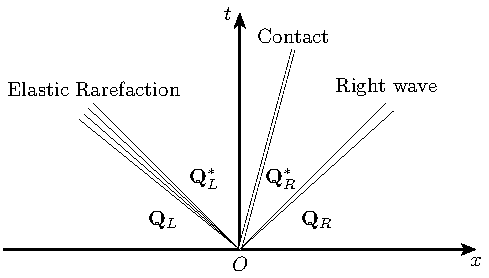
\includegraphics[width=3.8cm]{Tikz-figure0.eps}}
  \subfigure[Plastic rarefaction wave]{
	\label{fig:subfigure:b}
  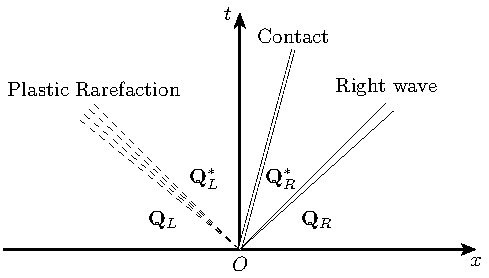
\includegraphics[width=3.8cm]{Tikz-figure1.eps}}
  \subfigure[Both elastic and plastic rarefaction waves]{
	\label{fig:subfigure:c}
  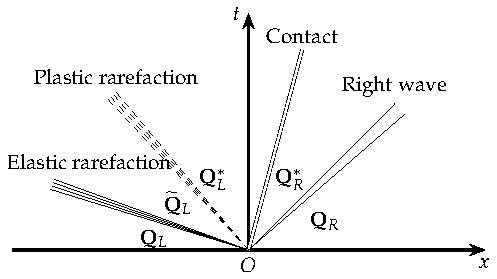
\includegraphics[width=3.8cm]{Tikz-figure2.eps}}
  \subfigure[ Elastic shock wave]{
	\label{fig:subfigure:d}
  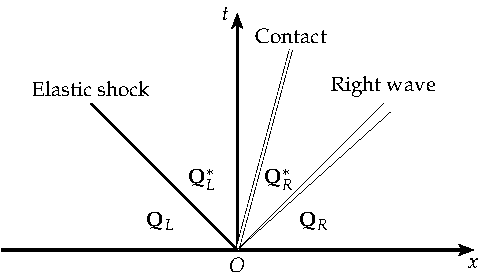
\includegraphics[width=3.8cm]{Tikz-figure3.eps}}
  \subfigure[Plastic shock wave]{
	\label{fig:subfigure:e}
  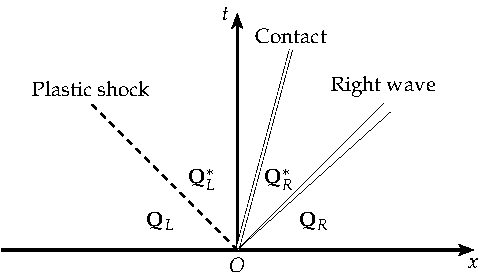
\includegraphics[width=3.8cm]{Tikz-figure4.eps}}
  \subfigure[Both elastic and plastic shock waves]{
	\label{fig:subfigure:f}
	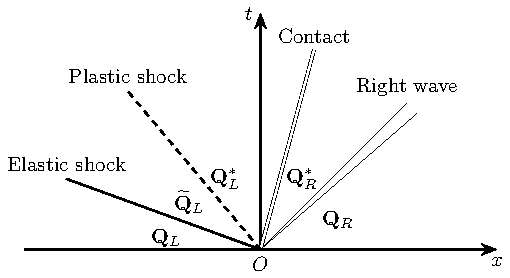
\includegraphics[width=3.8cm]{Tikz-figure5.eps}}
  \caption{The possible cases of Riemann solution structures in the left side.}
  \label{fig:cases}
\end{figure}

There are mainly three parts in the soluting process. 

Firstly, a pre-evaluation need to  be done to detect the left cases in Fig.\ref{fig:cases} and the corresponding right cases. This is done in Section (\ref{sec:eva}) with shock-contact-shock waves assumption.  

Secondly, for the cases with two waves in one side (i.e.  case c and case f in Fig.\ref{fig:cases}),we need to  solve  the states in the region $\tilde{\mathbf{Q}}_L$ and $\tilde{\mathbf{Q}}_R$. This is done in Section \ref{sec:tilde}.

At last,   we know all  the states besides $Q^*_L$ and $Q^*_R$. According to the knowledge in Section \ref{sec:rarefaction} and Section \ref{sec:shock}, if we  know the densities $\rho^*_L$ and $\rho^*_R$, we can solve all other unknowns out.
Also, by the informations in Section \ref{sec:contact}, the velocities and the Cauchy stresses  in the two sides of the contact must be equal. So there are two equations 
\begin{equation}\label{eq:fus}
  \begin{align}
	f_u(\rho^*_L,\rho^*_R) = u_L^* -u_R^* = 0,\\
	f_\sigma(\rho^*_L,\rho^*_R) = \sigma_L^* -\sigma_R^* = 0,
\end{align}
\end{equation}
and two unknowns $\rho_L^*$ and $\rho_R^*$. Equation (\ref{eq:fus}) is implicit, we have use a Newton iteration method to solve it, this process is given in Section \ref{sec:iteration}. The details of $f_u$ and $f_\sigma$ are listed in Section \ref{sec:fufs}.
\subsection{Pre-evaluation and case classfication}\label{sec:eva}
At first, we assume that there are only one shock wave in the left side and one shock in the right side as shown in Fig.\ref{fig:HLLC}. According to the conservation relations across the shocks, we have    
\begin{equation}
  \left\{
  \begin{align}
	\hat{\rho}_L\hat{u}^*_L = \rho_L u_L +s_L(\hat{\rho}_L^*-\rho_L), \\
	\hat{\rho}_L\hat{u}_L^{*2}-\sigma_L^* = \rho_L u_L^2 -\sigma_L +s_L(\hat{\rho}_L^* \hat{u}_L^*-\rho_L u_L), \\
  \end{align}
\right.
\end{equation}
and
\begin{equation}
  \left\{
  \begin{align}
	\hat{\rho}_R\hat{u}^*_R = \rho_R u_R +s_R(\hat{\rho}_R^*-\rho_R), \\
	\hat{\rho}_R\hat{u}_R^{*2}-\sigma_R^* = \rho_R u_R^2 -\sigma_R +s_R(\hat{\rho}_R^* \hat{u}_R^*-\rho_R u_R). \\
  \end{align}
\right.
\end{equation}

Using the relation across the interface,
\begin{equation}
  \hat{u}_L^* = \hat{u}_R^* =\hat{s}^*,\quad \hat{\sigma}_L^* = \hat{\sigma}_R^*.
\end{equation}
the speed of contact wave can be evaluated as 
\begin{equation}
\hat{s}^* = \frac{\sigma_L-\sigma_R+\rho_L u_L(s_L-u_L)-\rho_R u_R(s_R-u_R)}{\rho_L(s_L-u_L)-\rho_R(s_R-u_R)},
\end{equation}
the density is solved as 
\begin{equation}
\hat{\rho}_L^* = \frac{\rho_L(u_L-s_L)}{\hat{s}^*-s_L}, \quad
\hat{\rho}_R^* = \frac{\rho_R(u_R-s_R)}{\hat{s}^*-s_R}.
\end{equation}
The devaitoric stress is ecaluated as 
\begin{equation}  \label{sxx1}
  \hat{s}_{xxL}^*=-\frac{4}{3}\mu\text{ln}(\frac{\hat{\rho}_L^*}{\rho_L})+s_{xxL}, \quad   \hat{s}_{xxR}^*=-\frac{4}{3}\mu\text{ln}(\frac{\hat{\rho}_R^*}{\rho_R})+s_{xxR}.
\end{equation}
Here we define the speeds of left and right going waves as
 \begin{equation}
      s_L = \text{min} (u_L-c_L, u_R-c_R, 0),  \quad s_R = \text{max}(u_L+c_L, u_R+c_R, 0).
\end{equation}
By  the relation of $\hat{\rho}_{L(R)}$ and  $\hat{s}_{xxL(R)}$ we can classify every side into six cases, and conditions for the classfication are  shown in Table \ref{tab:cases}, the  subscripts $_L$ and  $_R$  are omitted for simplication. 

\begin{table}
  \centering 
  \caption{The condition of  cases classification.}
  \begin{tabular}{c|ccc}
	\toprule
	Conditions & $|s_{xx}|<\frac{2}{3}Y_0$ and $|\hat{s}_{xx}|<\frac{2}{3}Y_0$ & $s_{xx}=\frac{2}{3}Y_0$&  other\\
  \midrule
  $\hat{\rho^*} <\rho$ & case a& case b& case c \\
  $\hat{\rho^*} >\rho$ & case d& case e& case f \\
  \bottomrule
\end{tabular}
\label{tab:cases}
\end{table}

\subsection{State in region $\tilde{\mathbf{Q}}_{L(R)}$}\label{sec:tilde}


For cases (a,b,d,e) in Fig.\ref{fig:cases}, the material is totally yielding or totally not yielding, if we give a density $\rho_L^*$ in the region $\mathbf{Q}_L^*$, by the deductions in Section \ref{sec:rarefaction} and Section \ref{sec:shock}, all the unknowns in region $\mathbf{Q}_L^*$ can be solved out.

For cases (c,f), the meterial periods a yielding process from elastic to plastic. There is one more state $\tilde{\mathbf{Q}}_{L(R)}$ exists. In state $\tilde{\mathbf{Q}}_{L(R)}$, the derivative stress achieves the elastic limit 
\begin{equation}
  \tilde{s}_{xxL(R)} = \left\{ \begin{align}
	  &\frac{2}{3}Y_0 \quad  &\text{Case c},\\
	  &-\frac{2}{3}Y_0 \quad &\text{Case f},\\
	\end{align}
  \right.
\end{equation}
By (\ref{eq:rhosxx}), we can solve the density out as 
\begin{equation}
  \tilde{\rho}_{L(R)}= \left\{ \begin{align}
	  &\widetilde{\rho}_{L(R)} = \rho_{L(R)} \text{exp}\left(-\frac{Y_0}{2\mu}+\frac{3 s_{xxL(R)}}{4\mu}\right), \quad  & \text{Case c}, \\ 
	  &\widetilde{\rho}_{L(R)} = \rho_{L(R)} \text{exp}\left(\frac{Y_0}{2\mu}+\frac{3 s_{xxL(R)}}{4\mu}\right), \quad  & \text{Case f}. 
	\end{align}
  \right.
	\end{equation}
	As  the density in region $\mathbf{Q}^*_{L(R)}$ is known, all the pressure and velocity  can be solved by equations (\ref{eq:p_rho},\ref{eq:c_2rho},  \ref{eq:urho}) for a rarefaction wave  or by  equations (\ref{eq:shockp}, \ref{eq:shocku}) for a shock wave. 

	\subsubsection{Elastic rarefaction wave in case c}
	For case c, the pressure within the elastic rarefaction wave is 
	\begin{equation}
	  p(\rho) = p_{L(R)}e^{\frac{\lambda_1}{\rho_{L(R)}}-\frac{\lambda_1}{\rho}} +e^{-\frac{\lambda_1}{\rho}}\int_{\rho_{L(R)}}^{\rho} f_2(x) e^{\frac{\lambda_1}{x}}dx, \quad  \tilde{\rho}_{L(R)} \le \rho \le \rho_{L(R)}.
	\end{equation}
The sonic speed is 
	\begin{equation}
	c(\rho) =  \sqrt{ a_0^2 \frac{\partial f}{\partial \eta} + \frac{p(\rho)}{\rho^2}\rho_0\Gamma_0 -\frac{\rho_0}{\rho^2}\Gamma_0 s_{xx} +\frac{4}{3}\frac{\mu}{\rho}} \quad   \tilde{\rho}_{L(R)} \le \rho \le \rho_{L(R)}.
	\end{equation}
With the sonic speed, the velocity can be solved as
\begin{equation}
  u(\rho) = \left\{ \begin{aligned}
	u_L - \int_{\rho_L}^\rho \frac{c(x)}{x} dx,  \quad   \tilde{\rho}_L \le \rho \le \rho_{L} \\
	u_R + \int_{\rho_R}^\rho \frac{c(x)}{x} dx,  \quad   \tilde{\rho}_R \le \rho \le \rho_{R} \\
	\end{aligned}
  \right.
\end{equation}
So the pressure and velocity after the elastic wave are 
\begin{equation}
  \tilde{p}_{L(R)} = p(\tilde{\rho}_{L(R)}), \quad \tilde{u}_{L(R)} = u(\tilde{\rho}_{L(R)}).
\end{equation}

\subsubsection{Elastic shock wave in  case f}
For a shock wave (case f ), the pressure is 
\begin{equation}
  \tilde{p}_{L(R)}= \frac{2t(c_1f(\tilde{\rho}_{L(R)}/\rho_0)+e_L)-(\sigma_{L(R)}+\tilde{s}_{xxL(R)})}{2tc_0-1},
\end{equation}
where $c_0 = \frac{1}{\rho_0\Gamma_0}$ and $c_1 = \frac{a_0^2}{\Gamma_0}$ and $ t=\frac{\rho_{L(R)} \tilde{\rho}_{L(R)}}{\tilde{\rho}_{L(R)}-\rho_{L(R)}}$. 
And the velocity is 
\begin{equation}
  \tilde{u}_L = u_L -\sqrt{\frac{\sigma_L-\tilde{\sigma}_L}{t}},
\end{equation}
for the left, and 
\begin{equation}
  \tilde{u}_R = u_R +\sqrt{\frac{\sigma_R-\tilde{\sigma}_R}{t}},
\end{equation}
for the right-going wave.
	\subsection{Functions of velocity and Cauchy stress in region $\mathbf{Q}^*_{L(R)}$}\label{sec:fufs}
	The deductions of  velocity and Cauchy stress  for rarefaction waves and shocks are given in Section \ref{sec:rarefaction} and Section \ref{sec:shock}. For convenient, we list them in this section in  different cases. 
	\subsubsection{ $\mathbf{Q}^*_{L(R)}$ in  rarefaction wave cases }
	For rarefaction waves  in region
	The deviatoric stress is 
	\begin{equation}
	  s_{xxL(R)}^*= \left\{ \begin{aligned}
		  & s_{xxL(R)} \quad &\text{case (b, e)}, \\
		  & -\frac{4}{3}\mu\text{ln}\left(\frac{\rho_{L(R)}^*}{\rho_{L(R)}}\right)+s_{xxL(R)} \quad  &\text{case (a,d)},\\
		  & \frac{2}{3}Y_0 \quad  &\text{case (c)},\\
		  & -\frac{2}{3}Y_0 \quad &\text{case (f)}.\\
		\end{aligned}
	  \right.
	\end{equation}
The  pressure for case (a,b,c) is 
\begin{equation}
  p_{L(R)}^* = \left\{\begin{aligned}
	  &	p_{L(R)}e^{\frac{\lambda_1}{\rho_{L(R)}}-\frac{\lambda_1}{\rho_{L(R)}^*}} +e^{-\frac{\lambda_1}{\rho_{L(R)}^*}}\int_{\rho_{L(R)}}^{\rho_{L(R)}^*} f_2(x) e^{\frac{\lambda_1}{x}}dx. \quad & \text{case (a,b)},\\
	  &	\tilde{p}_{L(R)}e^{\frac{\lambda_1}{\tilde{\rho}_{L(R)}}-\frac{\lambda_1}{\rho_{L(R)}^*}} +e^{-\frac{\lambda_1}{\rho_{L(R)}^*}}\int_{\tilde{\rho}_{L(R)}}^{\rho_{L(R)}^*} f_2(x) e^{\frac{\lambda_1}{x}}dx. \quad & \text{case (c)},
  \end{aligned}
\right.
\end{equation} 
after get the pressure we can give the sonic speed as
\begin{equation}
  c_{L(R)}^{*2} = \left\{ \begin{aligned}
	&  a_0^2 \frac{\partial f}{\partial \eta} + \frac{p_{L(R)}^*}{\rho_{L(R)}^{*2}}\rho_0\Gamma_0 -\frac{\rho_0}{\rho_{L(R)}^{*2}}\Gamma_0 s_{xx} +\frac{4}{3}\frac{\mu}{\rho_{L(R)}^*} \quad & \text{case a},\\
	&	a_0^2 \frac{\partial f}{\partial \eta} + \frac{p}{\rho_{L(R)}^{*2}}\rho_0\Gamma_0 -\frac{\rho_0}{\rho_{L(R)}^{*2}}\Gamma_0 s_{xxL(R)}^*  \quad  & \text{case (b,c)}.
	\end{aligned}
  \right.
\end{equation}
then the velocity can be solved as
\begin{equation}
  u_{L}^* =\left\{ \begin{aligned} 
	  &u_L - \int_{\rho_L}^{\rho_L^*} \frac{c}{\rho} d\rho \quad \text{case a,b}, \\
	  &\tilde{u}_L - \int_{\tilde{\rho}_L}^{\rho_L^*} \frac{c}{\rho} d\rho \quad \text{case c}, \\
	\end{aligned}
  \right.
 u_{R}^* =\left\{ \begin{aligned} 
	 &u_R + \int_{\rho_R}^{\rho_R^*} \frac{c}{\rho} d\rho \quad \text{case a,b}, \\
	 &\tilde{u}_R + \int_{\tilde{\rho}_R}^{\rho_R^*} \frac{c}{\rho} d\rho \quad \text{case c}. \\
	\end{aligned}
  \right.
\end{equation}



  \subsection{An iteration process of $\rho^*_L$ and $\rho^*_R$}\label{sec:iteration}

  As the states in regions $\mathbf{Q}_L$ and $\mathbf{Q}_R$ are known, for cases (c,f) with two waves in one side, regions $\hat{\mathbf{Q}}_L$  and $\hat{\mathbf{Q}}_L$ are also solved in the above section, by the relaions in Section \ref{sec:rarefaction} and Section \ref{sec:shock}, if we know the densities $\rho_L^*$ and $\rho_R^*$, states in regions $\mathbf{Q}_L^*$ and $\mathbf{Q}_R^*$ can be deduced out. Till then, the  whole Riemann problem is solved.  

The Newton iteration to evaluate $\rho_L^*$ and $\rho_R^*$ is given as
\begin{equation}
\left[ \begin{array}{l}
 \rho _{L,(k+1)}^*\\
\rho_{R,(k+1)}^*\\
\end{array}
\right] = 
\left[ \begin{array}{l}
 \rho _{L,(k)}^*\\
\rho_{R,(k)}^*\\
\end{array}
\right]-
\left[ \begin{array}{ll}
\frac{\partial f_{u(k)}}{\partial \rho_L^*} & \frac{\partial f_{u(k)}}{\partial \rho_R^*}\\
\frac{\partial f_{\sigma(k)}}{\partial \rho_L^*} & \frac{\partial f_{\sigma(k)}}{\partial \rho_R^*}\\
\end{array}
\right]^{-1}
\left[ \begin{array}{l}
f_{u(k)}\\
f_{\sigma(k)}\\
\end{array}
\right]
\end{equation}

The initial of densities are given as the pre-evalation values,
\begin{equation}
  \rho_{L(0)}^* = \hat{\rho}_L \quad \rho_{R(0)}^* = \hat{\rho}_R.
\end{equation}
The  convergence is meassured by 
\begin{equation}
\text{CHA} = \text{max} \left[  
\frac{|\rho_{L(k+1)}^*- \rho_{L,(k)}^*|}{\frac{1}{2}|\rho_{L(k+1)}^*+\rho_{L(k)}^*|},   \frac{|\rho_{R(k+1)}^*- \rho_{R,(k)}^*|}{\frac{1}{2}|\rho_{R(k+1)}^*+\rho_{R(k)}^*|},|f_{u}|,|f_{\sigma}|\right].
\end{equation}
and the tolerance is taken as $\text{TOL} = 10^{-4}$. It usually takes 3-4 step to get a convergence result.

The derivatives of $f_{u}$ and $f_{\sigma}$ are given by
\begin{equation}
  \frac{\partial f_{u,(k+1)}}{\partial \rho^*_{L(R)}} = \frac{f_{u,(k+1)}-f_{u,(k)}}{\rho_{L(R),(k+1)}^* - \rho_{L(R),(k)}},\quad
  \frac{\partial f_{\sigma,(k+1)}}{\partial \rho^*_{L(R)}} = \frac{f_{\sigma,(k+1)}-f_{\sigma,(k)}}{\rho_{L(R),(k+1)}^* - \rho_{L(R),(k)}},
\end{equation}
At the first step, we use a simple  numerical difference  method
\begin{equation}
  \frac{\partial f_{u,(1)}}{\partial \rho^*_{L(R)}} = \frac{f_{u}(\rho^*_{L(R)}+\Delta \rho)-f_{u}(\rho^*_{L(R)})}{\Delta \rho_{L(R)}},\quad
  \frac{\partial f_{u,(1)}}{\partial \rho^*_{L(R)}} = \frac{f_{u}(\rho^*_{L(R)}+\Delta \rho)-f_{u}(\rho^*_{L(R)})}{\Delta \rho_{L(R)}},
\end{equation}
where $\Delta \rho$ is a little quatity, we can choose it as
\begin{equation}
  \Delta \rho_{L(R)} = \frac{\rho_{L(R),(0)}^*}{100}.
\end{equation}

A flow chat of this process is shown in Fig.


\subsection{Summary of MHLLCEP}
Here, we present all the procedures of MHLLCEP in a more simple way.
\begin{enumerate}
  \item  Assume  that there are three  waves in the Riemann solver. Based on this assumption, we perform the following evaluations:
  \begin{enumerate}
    \item evaluate  $\hat{s}^*$
    \begin{equation*}
       \hat{s}^* = \frac{\sigma_L-\sigma_R+\rho_L u_L(s_L-u_L)-\rho_R u_R(s_R-u_R)}{\rho_L(s_L-u_L)-\rho_R(s_R-u_R)}.
   \end{equation*}
    \item Evaluate  $\hat{\rho}_L^*$ and $\hat{\rho}_R^*$
    \begin{equation*}
       \hat{\rho}_L^* = \frac{\rho_L(u_L-s_L)}{s^*-s_L}, \hspace{0.3cm}  \hat{\rho}_R^* = \frac{\rho_R(u_R-s_R)}{s^*-s_R}.
    \end{equation*}
    \item Evaluate  the deviatoric stress
       \begin{equation*}
        \hat{s}_{xxL}^*=-\frac{4}{3}\mu\text{ln}(\frac{\hat{\rho}_L^*}{\rho_L})+s_{xxL},\hspace{0.2cm}  \hat{s}_{xxR}^*=-\frac{4}{3}\mu\text{ln}(\frac{\hat{\rho}_R^*}{\rho_R})+s_{xxR}.
      \end{equation*}
    \item Evaluate the pressure
  \end{enumerate}
  \item Decide whether the state reach the elastic limit or not
        \begin{enumerate}
          \item If $|s_{xxL}| < \frac{2}{3}Y_0 \le |\hat{s}_{xxL}^*| $, there are two waves exist in the left, we need to  evaluate the left yielding state.

          The deviatoric stress, density and pressure behind the left elastic  wave are given as
\begin{equation*}
  \widetilde{s}_{xxL} =\left\{ \begin{aligned}
      -\frac{2}{3}Y_0, \hspace{0.3cm} \text{if} \hspace{0.3cm} \rho_L^* > \rho_L,\\
      \frac{2}{3}Y_0, \hspace{0.3cm} \text{if} \hspace{0.3cm} \rho_L^* < \rho_L,\\
    \end{aligned}\right.
 \end{equation*}
 \begin{equation*}    
     \widetilde{\rho}_{L} = \left\{ \begin{aligned}
      & \rho_L \text{exp}\left(\frac{Y_0}{2\mu}+\frac{3 s_{xxL}}{4\mu}\right)  \hspace{0.5cm} \text{if} \hspace{0.3cm} \rho_L^* > \rho_L,\\
& \rho_L \text{exp}\left(-\frac{Y_0}{2\mu}+\frac{3 s_{xxL}}{4\mu}\right)
\hspace{0.3cm} \text{if} \hspace{0.3cm} \rho_L^* < \rho_L,\\
  \end{aligned}\right.
 \end{equation*}
 
\begin{equation*}
  \widetilde{p}_L= \frac{2t(c_1f(\widetilde{\rho}_L)+e_L)-(\sigma_L+\widetilde{s}_{xxL})}{2tc_0-1}, \hspace{0.3cm}
t=\frac{\rho_L \widetilde{\rho}_L}{\widetilde{\rho}_L-\rho_L},
\end{equation*}
and the Cauchy stress and velocity are
\begin{equation*}
\widetilde{\sigma}_L = -\widetilde{p}_L+\widetilde{s}_{xxL},
\end{equation*}
\begin{equation*}
  \widetilde{u}_L= \left\{
  \begin{aligned}
    u_L-\sqrt{\frac{\sigma_L-\widetilde{\sigma}_L}{t}} \hspace{0.2cm} \text{if} \hspace{0.2cm} \rho_L^* >\rho_L,\\
    u_L+\sqrt{\frac{\sigma_L-\widetilde{\sigma}_L}{t}} \hspace{0.2cm} \text{if} \hspace{0.2cm} \rho_L^* <\rho_L.\\
\end{aligned} \right.
\end{equation*}
If not,
\begin{equation*}
  \widetilde{\mathbf{Q}}_L = \mathbf{Q}_L.
\end{equation*}
          \item If $|s_{xxR}| < \frac{2}{3}Y_0 \le |\hat{s}_{xxR}^*| $, right  elastic and plastic wave exist, we need to  evaluate the right yielding state.

                           The deviatoric stress, density and pressure  behind the right elastic  wave are given as
\begin{equation*}
  \widetilde{s}_{xxR} =\left\{ \begin{aligned}
      -\frac{2}{3}Y_0, \hspace{0.3cm} \text{if} \hspace{0.3cm} \rho_R^* > \rho_R,\\
      \frac{2}{3}Y_0, \hspace{0.3cm} \text{if} \hspace{0.3cm} \rho_R^* < \rho_R,\\
    \end{aligned}\right.
    \hspace{0.2cm} \widetilde{\rho}_{R} = \left\{ \begin{aligned}
      & \rho_R \text{exp}\left(\frac{Y_0}{2\mu}+\frac{3 s_{xxR}}{4\mu}\right)  \hspace{0.5cm} \text{if} \hspace{0.3cm} \rho_R^* > \rho_R,\\
& \rho_R \text{exp}\left(-\frac{Y_0}{2\mu}+\frac{3 s_{xxR}}{4\mu}\right)
\hspace{0.3cm} \text{if} \hspace{0.3cm} \rho_R^* < \rho_R,\\
  \end{aligned}\right.
 \end{equation*}
\begin{equation*}
  \widetilde{p}_R= \frac{2t(c_1f(\widetilde{\rho}_R)+e_R)-(\sigma_R+\widetilde{s}_{xxR})}{2tc_0-1}, \hspace{0.3cm}
t=\frac{\rho_R \widetilde{\rho}_R}{\widetilde{\rho}_R-\rho_R},
\end{equation*}
and the Cauchy stress and velocity are
\begin{equation*}
\widetilde{\sigma}_R = -\widetilde{p}_R+\widetilde{s}_{xxR},
\end{equation*}
\begin{equation*}
  \widetilde{u}_R= \left\{
  \begin{aligned}
    u_R+\sqrt{\frac{\sigma_R-\widetilde{\sigma}_R}{t}} \hspace{0.2cm} \text{if} \hspace{0.2cm} \rho_R^* >\rho_R,\\
    u_R-\sqrt{\frac{\sigma_R-\widetilde{\sigma}_R}{t}} \hspace{0.2cm} \text{if} \hspace{0.2cm} \rho_R^* <\rho_R.\\
\end{aligned} \right.
\end{equation*}
If not,
\begin{equation*}
  \widetilde{\mathbf{Q}}_R = \mathbf{Q}_R.
\end{equation*}

        \end{enumerate}
  \item Re-evaluate the states in the star regions on both sides of the contact wave
  \begin{enumerate}
    \item Evaluate the wave speeds:
\begin{equation*}
  s_L = \text{min} (\widetilde{u}_L-\widetilde{c}_L, \widetilde{u}_R-\widetilde{c}_R,0), \hspace{0.3cm} s_R = \text{max}(\widetilde{u}_L+\widetilde{c}_L, \widetilde{u}_R+\widetilde{c}_R,0),
    \end{equation*}
    \begin{equation*}
      s^* = \frac{\widetilde{\sigma}_L-\widetilde{\sigma}_R+\widetilde{\rho}_L \widetilde{u}_L(s_L-\widetilde{u}_L)-\widetilde{\rho}_R \widetilde{u}_R(s_R-\widetilde{u}_R)}{\widetilde{\rho}_L(s_L-\widetilde{u}_L)-\widetilde{\rho}_R(s_R-\widetilde{u}_R)}.
\end{equation*}

    \item Evaluate the densities:
\begin{equation*}
  \rho_L^* = \frac{\widetilde{\rho}_L(\widetilde{u}_L-s_L)}{s^*-s_L}, \hspace{0.3cm}  \rho_R^* = \frac{\widetilde{\rho}_R(\widetilde{u}_R-s_R)}{s^*-s_R},
\end{equation*}

    \item Evaluate the deviatoric stresses:
 \begin{align*}
   \widetilde{s}_{xxL}^* = \left\{\begin{array}{cc}
                       \widetilde{s}_{xxL} & if \ |\hat{s}_{xxL}^{*}|\geq \frac{2}{3}Y_{0} \\
                        -\frac{4}{3}\mu \text{ln}\left( \frac{\rho_L^*}{\widetilde{\rho}_L}  \right)+\widetilde{s}_{xxL} & otherwise
                     \end{array}\right.
   ,\\
   \widetilde{s}_{xxR}^* =  \left\{\begin{array}{cc}
                       \widetilde{s}_{xxR} & if \ |\hat{s}_{xxR}^{*}| \geq \frac{2}{3}Y_{0} \\
                        -\frac{4}{3}\mu \text{ln}\left( \frac{\rho_R^*}{\widetilde{\rho}_R}  \right)+\widetilde{s}_{xxR} & otherwise
                     \end{array}\right.
    ,
\end{align*}
then using  the von Mises' yielding condition
\begin{equation*}
  s_{xxL}^* = \Upsilon(\widetilde{s}_{xxL}^*) , \hspace{0.3cm}  s_{xxR}^* = \Upsilon(\widetilde{s}_{xxR}^*).
\end{equation*}

    \item Solving the Cauchy stresses:
\begin{equation*}
  \sigma_L^*=\sigma_R^*=\widetilde{\sigma}_L -\widetilde{\rho_L} (s_L-\widetilde{u}_L)(s^*-\widetilde{u}_L).
\end{equation*}

     \item The pressure is given by $p =s_{xx}-\sigma$.
  \end{enumerate}
\end{enumerate}

\end{document}
